
\section{Single cells analysis}
\label{chap:UnitsAnalysis}
%Neurons in VS and VTA were classified in cell-types.
%In order to understand how specific interregional interaction between VS and VTA are involved in reward prediction signal (RPE) we used 
%The aim of the project is to understand the nature of interactions between ventral striatum (VS) and ventral tegmental area (VTA). Loops and circuit effects make puzzling to understand the whole picture of the aforementioned interactions (figure\ref{fig:Brain}, left). To see how specific interactions are involved in the prediction coding is needed a cell-types classification of underlying units.\\
In this chapter we present the cell-types classification of VS and VTA units provided by Max Scheller, that was later entered in our analysis to understand specifically which cell-types were involved in interregional interactions and whether interregional interactions formed by different cell-types were involved in different aspects of the reward-related signals. Figure \ref{fig:Brain} shows a schematic representation of VS-VTA circuit, with subregions and cell-types used in this study.\\
\begin{figure}[H]
    \centering
    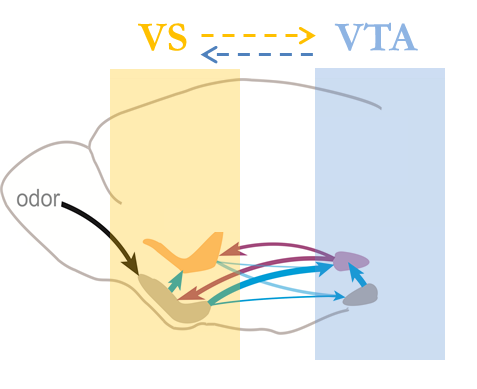
\includegraphics[width=0.45\textwidth]{BrainVSVTA.png}
    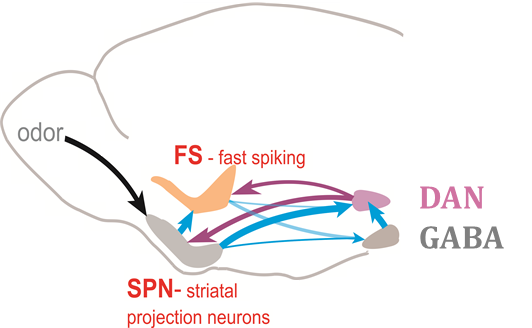
\includegraphics[width=0.45\textwidth]{Brain.png}
    \caption{Schematic illustration of VS-VTA regions and their interactions in mice brain. On the left the mesoscopic vision, VS in yellow is subdivided in odor tuberculum (OT) and nucleus accumbens (NAcc), neurons of VS both project into VTA and receive inputs from VTA. On the right the detailed vision, with specification of the recorded cell-types involved in VS-VTA circuit.}
    \label{fig:Brain}
\end{figure}
The data-set included $803$ VS and pallidal units and $272$ VTA units in total, further classified in cell-types. Specifically VS units were classified as either striatal projection neurons (SPNs), fast-spiking neurons (FSNs) or cholinergic interneurons (CINs) according to their firing pattern characteristics computed using only spikes during the inter-trials interval and after session. Units with a firing rate higher than 12 Hz were assigned as FSNs and all units with a firing rate below 2 Hz as SPNs. Units in the remaining range were designed as putative regular-firing CINs if the coefficient of variation (CV) of their ISI distribution was less than 1.2 and ISIs less than 60 ms contributed no more than 20$\%$ of all ISIs (\cite{Inokawa}). Finally the resting units were characterized as SPNs or FSNs if they ever were silent for more than 2 seconds (\cite{Graybiel}). Using this classification, mean normalized autocorrelations and mean waveforms have canonical patterns.\\The VS consists of the nucleus accumbens and the olfactory tubercle (OT). Considering the close anatomical relationship between OT and VP (\cite{Heimer1982}), and  the fact that 95$\%$ of the neurons in striatum are SPNs with baseline firing rates below 5 Hz (\cite{Kravitz}); we considered all single units with baseline firing $> 10$ Hz as putative ventral pallidal FSN.\\VTA units were instead classified as dopaminergic neurons (DAN), gabaergic units (GABA), and glutamatergic neurons (GLU) according to their task related activity using a clustering approach adapted from \cite{Uchida}. First, response were characterized for the relevant time spans (CS+ from 0 to 0.5 and US from -0.5 to 0 and from 0 to 0.5), significant task related response were assessed with Friedman test, and only significant units ($p<0.05$) were included in the clustering classification ($~80\%$ of units).\\For the clustering of US-responsive units, the spike count distribution were used to construct one trace per neuron by computing auROC-values analogously to the Friedman significant test, yielding a trace of values between 0 and 1. Where 0.5 means no distinguishability between test and control distribution. Hierarchical clustering was done on these traces using the in-built linkage matlab function.\\Figure \ref{fig:ClassificatonVTA} displays the VTA units classification. In this study we focused on DAN and GABA in assemblies. DAN fire phasic to the reward and/or to the rewarded stimulus, whereas GABA units are tonically active.
\begin{figure}[H]
  \centering
    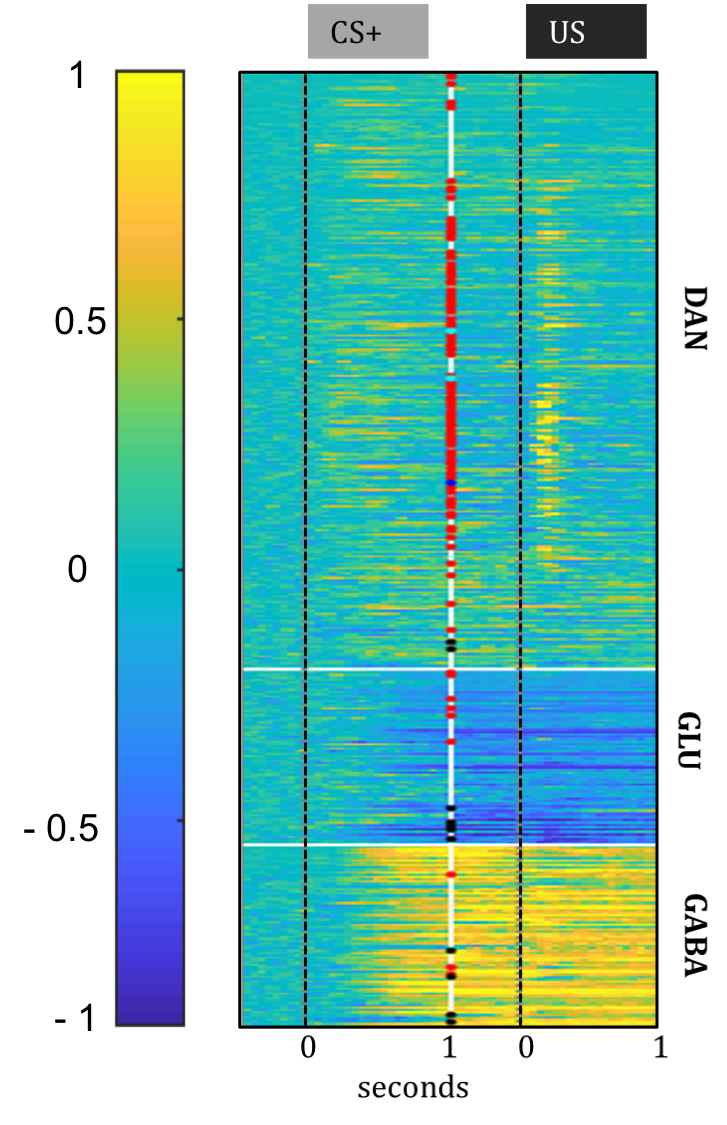
\includegraphics[scale=0.5]{figures/VTA_CellClass.png}
    %\hspace{1cm}
    %
\includegraphics[scale=0.55]{figures/parula1.png}
   \caption{Figure provided by Max Scheller. VTA classification according to units task related activity using a clustering approach adapted from \cite{Uchida}. After normalization and subtraction of the mean of the baseline, the activity range from -1 to 1; activity plot colors range from dark blue to yellow. Where dark blue means an inhibition with respect to the baseline and yellow indicates an activation. In this study we focused on dopaminergic and gabaergic units in assemblies. DAN fire phasic to the reward and/or to the rewarded stimulus, whereas GABA are tonically active.}
    \label{fig:ClassificatonVTA}
\end{figure}
Considering the units recorded in paradigms used for the assembly analysis, different cell-types occurred with different frequency. SPN were the most frequent unit types in VS ($\sim55\%$), followed by FSN in VP ($\sim42\%$). We recorded few CIN ($\sim2\%$), and only the $1\%$ c. were not classified units. In VTA the DAN were the most frequent cell-types ($\sim45\%$), followed by the GABA ($\sim19\%$) and the GLU ($\sim7\%$). The $29\%$ c. of units were not classified. Figure \ref{fig:PieRegions} shows the cell-types occurrence in VS and VTA.
\begin{figure}[H]
  \centering
    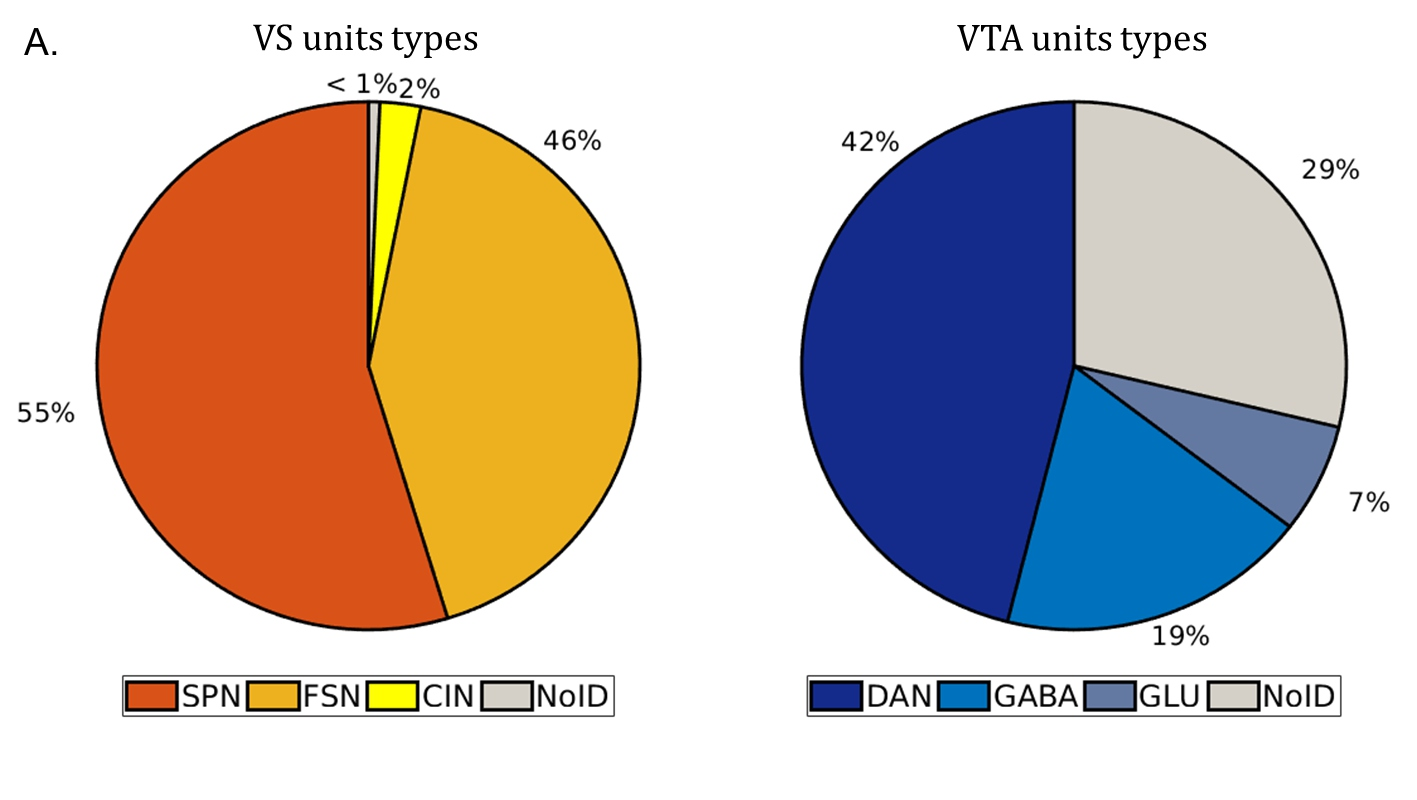
\includegraphics[scale=0.5]{figures/PieRegions1.pdf}
   \caption{Left: units types pie chart in VS. Right: units types pie chart in VTA}
    \label{fig:PieRegions}
\end{figure}

